\section{Simetría, periodicidad y continuidad del espectro $\Sigma_{x}$}
\label{sec: simetria, periodicidad, continuidad}
Fijada una dimensión $n \geq 2$,
si $x \in \IR^{n}$ es cualquier señal y 
$\Sigma_{x}$
es su espectro como se definió en
\ref{def: espectro monofrecuenciales},
en esta sección vamos a demostrar 
algunos resultados sobre la periodicidad 
de esta función y su simetría 
respecto a puntos de la forma
$\frac{n}{2} \IZ$.
Esto será de utilidad pues nos permitirá
acotar considerablemente el dominio de frecuencias
de $\Sigma_{x}$.



\begin{prop}
\label{prop: periodicidad espectro}
\textbf{(Periodicidad del espectro)}
Sean $n \geq 2$, $x \in \IR^{n}$.
Sea $\Sigma_{x}$ el espectro de $x$ como se definió en 
\eqref{def: espectro monofrecuenciales inicial}.
El espectro $\Sigma_{x}$ es $n-$periódico, es decir, 
para cualquier frecuencia
$0 \leq \omega \leq n$
y toda $K \in \IZ$, se tiene que 
\[
\sigma_{n}(x, \omega) = \sigma_{n}(x, \omega + Kn).
\]
\end{prop}
\noindent
\textbf{Demostración.}
Sólo observe que 
\begin{align*}
\tilde{c}_{n, \omega + Kn} = & \left( cos \left( 2 \pi
\left( \omega + Kn \right) \frac{m}{n} \right) \right)_{m=0}^{n-1} \\
= & \left( cos \left( 
2 \pi \omega \frac{m}{n} + 2 \pi K m
\right) \right)_{m=0}^{n-1} \\
= & \left( cos \left( 
2 \pi \omega \frac{m}{n}
\right) \right)_{m=0}^{n-1} = \tilde{c}_{n, \omega}
\end{align*}
y, similarmente, que 
\[
\tilde{s}_{n, \omega + Kn} = \tilde{s}_{n, \omega},
\]
luego, por definición de los espacios monofrecuenciales
(c.f. ecuación \ref{eq: espacio Pnw}),
\begin{align*}
P_{n, \omega + Kn} =
& span(\tilde{c}_{n, \omega + Kn}, \tilde{s}_{n, \omega + Kn}) \\
= & span(\tilde{c}_{n, \omega }, \tilde{s}_{n, \omega }) = P_{n, \omega};
\end{align*}
de esto se concluye, usando la definición
\ref{def: final de sigmas},
que 
\[
\sigma_{n}(x, \omega) = 
cos (\measuredangle(x, P_{n, \omega}))
= cos (\measuredangle(x, P_{n, \omega + Kn})) = 
\sigma_{n}(x, \omega + Kn).
\]
\QEDB
\vspace{0.2cm}

\begin{figure}[H]
	\sidecaption{
	Según la periodicidad establecida en la proposición 
	\ref{prop: periodicidad espectro}, basta calcular los
	coeficientes espectrales
	$\sigma_{n}(x, \omega)$ para frecuencias
	$0 \leq \omega \leq n$.
	\label{fig: periodicidad espectro}
	}
	\centering
	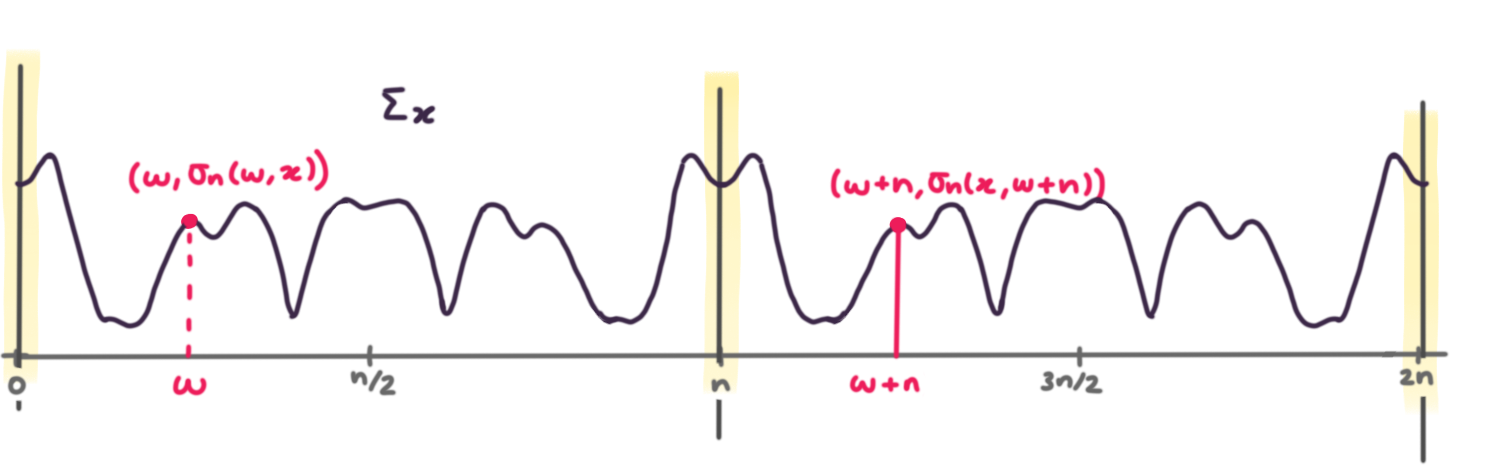
\includegraphics[scale = 0.9]{periodicidad_espectro} 
\end{figure}	


\begin{prop}
\textbf{(Simetría del espectro)}
Sean
$n \geq 2$,
$x \in \IR^{n}$. Para toda $0 \leq1 \omega \leq \frac{n}{2}$,
\[
\sigma_{n}(x, \omega) = 
\sigma_{n}(x, n-\omega ). 
\]
\end{prop}
\noindent
\textbf{Demostración.}
En efecto, 
\begin{align*}
\tilde{c}_{n, \omega + n} = & \left( cos \left( 2 \pi
\left( n- \omega \right) \frac{m}{n} \right) \right)_{m=0}^{n-1} \\
= & \left( cos \left( 
2 \pi n \frac{m}{n} - 2 \pi \omega
\frac{m}{n}
\right) \right)_{m=0}^{n-1} \\
= & \left( cos \left( 
2 \pi m - 2 \pi \omega \frac{m}{n} 
\right) \right)_{m=0}^{n-1} \\
= & \left( cos \left( 2 \pi \omega \frac{m}{n} \right) \right)_{m=0}^{n-1}
= \tilde{c}_{n, \omega}
\end{align*}
y, similarmente,
\[
\tilde{s}_{n, \omega + Kn} = -\tilde{s}_{n, \omega};
\]
de esto, como en la demostración de la proposición
\ref{prop: periodicidad espectro}, se concluye la igualdad
entre los espacios $P_{n, \omega}$ y $P_{n, n-\omega}$, y de esto
la igualdad deseada.
\QEDB
\vspace{0.2cm}

\begin{figure}[H]
	\sidecaption{
	Podemos así afinar la afirmación hecha en la figura 
	\ref{fig: periodicidad espectro} y concluir que basta
	calcular los coeficientes
	$\sigma_{n}(x, \omega)$ para $0 \leq \omega \leq \frac{n}{2}$,
	pues los demás pueden deducirse a partir de reflexiones y traslaciones.
	\label{fig: simetria espectro}
	}
	\centering
	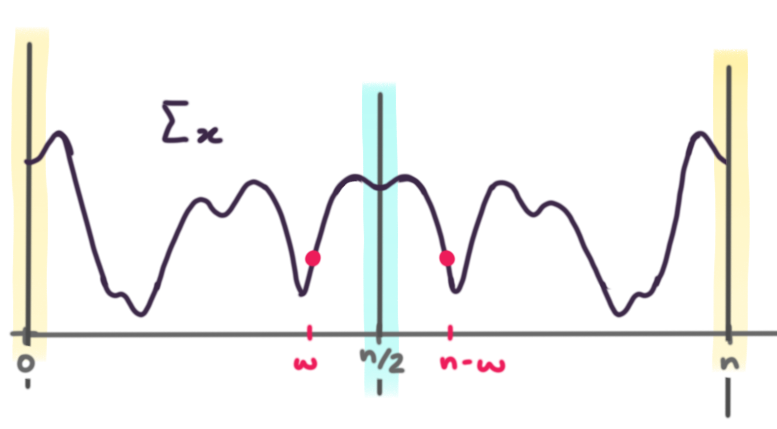
\includegraphics[scale = 1.4]{simetria_espectro} 
\end{figure}	
 

\begin{nota}
\label{nota: muestreo dom frecuencia}
Según estas propiedades de periodicidad y simetría,
podemos limitarnos a evaluar el espectro
$\Sigma_{x}$ de una señal sólo en frecuencias
contenidas en el intervalo $[0, n/2]$, pues los valores
del espectro para otros valores pueden deducirse por periodicidad
y simetría. \\

Ahora bien, para poder escribir programas
para calcular un tal espectro $\Sigma_{x}$
se debe de usar
un conjunto discreto de puntos.
Para los espectros que calcularemos de ahora en 
adelante, adoptamos la convención de 
usar usar como dominio 
del espectro
$\Sigma_{x}$ de una señal $x \in \IR^{n}$
al conjunto
\TODO{revisa!}
\begin{equation}
\label{eq: malla frecuencias}
\left\{ \frac{a}{100} : \hspace{0.2cm}
0 \leq a \leq \frac{100n}{2} \right\},
\end{equation}

es decir, se toman $100$ muestras por
cada unidad del intervalo 
$\left[ 0, \frac{n}{2}\right]$
\end{nota}


Para terminar, hagamos algunos comentarios
sobre la continuidad del espectro $\Sigma_{x}$
de una señal $x \in \IR^{n}$. \\
Por definición del espectro, 
si $\omega \geq 0$, entonces
$\Sigma_{x}(\omega) = \sigma_{n} (x, \omega)$,
donde los coeficientes
$\sigma_{n} (x, \omega)$ son como se definieron en
la proposición \ref{prp: ammm}.
Por la periodicidad y simetría del espectro, basta
analizar la continuidad de $\Sigma_{x}$ sólo en el
intervalo cerrado $[0, n/2]$. \\

Observe que la fórmula
\eqref{eq: coef sigma caso 1}, que sirve
para calcular $\sigma_{n} (x, \omega)$
cuando $\omega \in ]0, n/2[$, es una combinación
de sumas y productos de senos y cosenos
evaluados en funciones de la frecuencia $\omega$, luego, 
es una función continua, por lo tanto $\Sigma_{x}$
es continua en el interior del intervalo 
$[0, n/2]$. No pudimos determinar la
continuidad de $\Sigma_{x}$ en los puntos
extremos $0$ y $n/2$, ni encontramos un criterio que deba
cumplir la señal que implique la continuidad en uno
de estos puntos extremos.
No escribimos en detalle los intentos para
determinar los límites
\[
\limite{\omega \rightarrow 0^{+}}{\sigma_{n}(x, \omega)}
\hspace{0.2cm} \textit{y} \hspace{0.2cm}
\limite{\omega \rightarrow \frac{n}{2}^{-}}{\sigma_{n}(x, \omega)},
\]
pero comentamos que el problema que encontramos fue
intentar determinar el límite
(cuando $\omega \rightarrow 0^{+}$ y cuando $\omega \rightarrow \frac{n}{2}^{-}$)
de la expresión
\[
\sqrt{2} \left(
n - \frac{sen(2 \pi \omega) cos (2 \pi \omega \frac{n-1}{n})}{sen(2 \pi \omega/n)}
\right)^{-1/2}
\cdot
\suma{m=0}{n-1}{x_{m} sen(2 \pi \omega m/n)};
\]
puesto que se tiene una indeterminación de tipo
$\infty \cdot 0$, se aplicó la Regla de L'Hôpital
(c.f. \cite{hopital}) 
para intentar determinar el límite, pero esto sólo
nos llevó a una expresión más complicada que presentaba una indeterminación
de tipo $\frac{0}{0}$. No esperabamos que la tarea
de determinar la continuidad por los extremos fuese sencilla,
pues después de graficar algunos espectros notamos que algunos
de ellos eran continuos por ambos extremos, mientras que otros
presentaban discountinuidades (que, por estár acotados los valores
del espectro por $0$ y $1$, necesariamente son de salto)
en uno o ambos extremos, y no notamos características de 
la señal $x$ a partir de la cual se calcula el espectro
que indicaran cuándo se tenía la discontinuidad por uno 
de los puntos extremos.





\section{Relación entre los espectros basados en la TDF y en espacios monofrecuenciales}

Después de todo lo expuesto en las secciones anteriores, tenemos
ya dos alternativas para realizar un análisis
espectral de una señal $x \in \IR^{n}$.

Sean $n \geq 2$, $M := \lceil \frac{n}{2} \rceil$, $x \in \IR^{n}$.
\begin{itemize}
	\item \textbf{(Espectro-0: basado en la TDF)} 
	Usando la transformada discreta de Fourier
	(c.f. sección \ref{sec: TDF}),
	el espectro de $x$ es la función
	\[
	\Tau_{x}: Dom_{TDF, n} \longrightarrow \IR^{+}_{0}
	\]	
	definida en \ref{def: espectro DFT}.
	
	La gráfica es entonces la de las frecuencias
	enteras $\omega$ dadas (dependiendo de la 
	paridad de $n$) por las
	tablas 6.1 y 6.2
	versus los coeficientes
	$\tau_{n}(x, \omega)$ definidos en
	\ref{def: taus}.
	
	Puesto que el realizar un análisis de 
	$x$ via la TDF significa encontrar una
	expresión de $x$ como una suma
	ponderada de muestreos de senos y cosenos,
	de frecuencias enteras las indicadas en las tablas 6.1 o 6.2,
	se tiene que  
	\begin{itemize}
		\item Para toda frecuencia $\omega$ considerada
		por la TDF,
		\[
		0 \leq \tau_{n}(x, \omega) \leq 1,
		\]
		y que
		\item entre más se acerque
		$\tau_{n, \omega}(x)$
		a $1$, mayor es la
		importancia de la frecuencia $\omega$ para
		sintetizar s $x$; recíprocamente, si 
		$\tau_{n}(x, \omega)$ es cercana a cero, entonces
		la frecuencia $\omega$ no es muy relevante para 
		sintetizar a la señal $x$.
	\end{itemize}
	\begin{defi}
	\label{def: FM0}
	Llamaremos \textbf{frecuencia principal-0}
	(y denotaremos por $FP0(x)$) 
	a una 
	frecuencia $\omega \in Dom_{TDF, n}$
	tal que, para cualquier otra $\omega' \in Dom_{TDF, n}$ 
	se tenga que 
	\[
	\tau_{n}(x, \omega') = \Tau_{x}(\omega^{'}) \leq
	\Tau_{x}(\omega) =  
	 \tau_{n}(x, \omega).
	\]
	\end{defi}
	Observe que tal frecuencia principal existe por ser 
	el máximo de un conjunto finito de números, pero que no 
	estamos asegurando que sea única. 
	
	\item \textbf{(Espectro-1: basado en espacios monofrecuenciales)} 
	Usando
	las ideas propuestas en 
	la sección
	\ref{sec: metodologia para realizar un analisis espectral que considere frecuencias arbitrarias}, 
	es decir, si se usan cosenos de ángulos a
	espacios monofrecuenciales $P_{n, \omega}$
	(c.f. \ref{eq: espacio Pnw}), el espectro
	de una señal $x$ se definió en
	\ref{def: espectro monofrecuenciales inicial}
	como la función 
	\[
	\Sigma_{x} : \left[0, \frac{n}{2} \right] \longrightarrow [0,1].
	\]
	
	La gráfica de este espectro es la de 
	las frecuencias $\omega \in [0, \frac{n}{2}]$ versus	
	los coeficientes
	$\sigma_{n}(x, \omega)$ definidos en 
	\ref{prp: ammm}. Observe que
	\begin{itemize}
		\item para cualquier frecuencia $\omega \geq 0$, se tiene que
		\[
		0 \leq \sigma_{n}(x, \omega) \leq 1
		\]
		\item 
	y, el que
	$\sigma_{n}(x, \omega)$ sea cercano a $1$ significa que un
	muestreo uniforme de un sinusoide de frecuencia $\omega$
	modela bien el comportamiento de $x$,
	mientras que un $\sigma_{n}(x, \omega)$ cercano
	a cero significa que 
	$x$ es casi perpendicular a toda señal de frecuencia $\omega$
	(c.f. nota \ref{nota: significado de los sigma en AE}).
	\end{itemize}
\end{itemize}

Nos gustaría, así como hicimos en la definición
\ref{def: FM0}, definir la frecuencia principal 
de una señal $x$ basada en el espectro
$\Sigma_{x}$ de esta. No es tan sencillo hacer esto, pues,
como comentamos en la sección
\ref{sec: simetria, periodicidad, continuidad}, no parece
que para toda señal $x \in \IR^{n}$ el espectro
$\Sigma_{x}$ sea continuo en los puntos extremos
$0$ y $n/2$, por lo que intentar definir una
frecuencia principal como
\[
\omega \in [0, n/2] \textit{ tal que }
a_{x} = \Sigma_{x}(\omega), \textit{ donde }
a_{x} = sup \{ \Sigma_{x}(w): \hspace{0.2cm} \omega
\in [0, n/2] \}
\]
no es adecuado, pues no está excluida la 
posibilidad de que exista un espectro $\Sigma_{x}$
para el que no exista una $\omega \in [0, n/2]$ 
tal que $\Sigma_{x}(\omega) = a_{x}$, o sea, tal que 
$a_{x}$ que no sea máximo
del conjunto 
$\{ \Sigma_{x}(w): \hspace{0.2cm} \omega
\in [0, n/2] \}$. \\

\begin{figure}[H]
	\sidecaption{
	Se muestra un dibujo hipotético de un espectro
	$\Sigma_{x}$ para el que $a_{x} = 1$ pero no exista
	ninguna frecuencia $\omega \geq 0$ (una candidata
	a frecuencia principal) tal que $\Sigma_{x}(\omega) = a_{x}$.
 	\label{fig: ej FP1}
	}
	\centering
	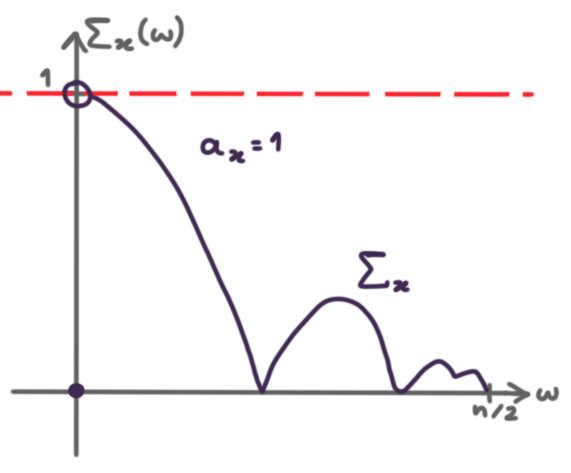
\includegraphics[scale = 1]{ejemplo_FP1.png} 
\end{figure}	
Sorteamos este problema si restringimos las frecuencias
$\omega$ a considerar a un subconjunto finito del
rango inicial de frecuencias
$[0, n/2]$.

\begin{defi}
	\label{def: FM1}
	Sean $n \geq 2$, $x \in \IR^{n}$. Sea
	$\cali{P}$ un subconjunto finito
	de $[0, n/2]$.
	Llamaremos la \textbf{frecuencia principal-$1$}
	(y denotaremos
	por $FP1(x)$) 
	de $x$ respecto al conjunto $\cali{P}$	
	a una frecuencia $\omega \in \cali{P}$ 
	tal que, para cualquier otra $\omega'$ del $\cali{P}$, se tenga que
	\[
	\sigma_{n, \omega'}(x) = \Sigma_{x}(\omega') 
	\leq \Sigma_{x}(\omega) = \sigma_{n, \omega}(x).
	\]
\end{defi}
En la práctica, el que se tenga que fijar un conjunto
finito $\cali{P} \subseteq [0, n/2]$ de frecuencias
para calcular la FP1 no es un problema, pues ya teníamos que hacer
esto para calcular, de forma computacional, el espectro
$\Sigma_{x}$. Para respetar la convención
puesta en la nota 
\ref{nota: muestreo dom frecuencia}, vamos
a tomar a $\cali{P}$ como en 
\eqref{eq: malla frecuencias}.
	
\begin{nota}
Observe que no estamos asegurando
que las frecuencias principales
$FP0(x)$ y $FP1(x)$ como se definieron en 
\ref{def: FM0} y \ref{def: FM1}
sean únicas.
Si hay dos o más frecuencias $\omega'$ que satisfagan
la definición de frecuencia principal-0 
(resp. frecuencia principal-1), tomamos
como valor de $FP0(x)$ 
(resp. $FP1(x)$)
a la mayor de tales $\omega'$.
\end{nota}


Demostremos ahora que, de hecho, el espectro-0
de hecho es la restricción del espectro-1
al conjunto de frecuencias 
$Dom_{TDF, n}$ considerado por la transformada discreta
de Fourier.
\begin{prop}
\label{prop: coinciden espectr}
Sean $n \geq 2$, $x \in \IR^{n}$.
Sea $Dom_{TDF, n}$ el dominio del espectro-0 de $x$
como se definió en \ref{def. Dom tdf}. Se tiene que
\begin{equation}
\label{eq4: 4May}
\forall \omega \in Dom_{TDF, n}:
\hspace{0.2cm} \tau_{n}(x, \omega) = \sigma_{n}(x, \omega).
\end{equation}
\end{prop}

\noindent
\textbf{Demostración.}
Recuerde que los coeficientes
$\sigma_{n}(x, \omega)$
se definieron como
\[
\sigma_{n}(x, \omega) = \frac{|| \Pi_{P_{n, \omega}}(x) ||}{|| x ||}.
\]
Teniendo una base ortonormal del espacio 
$P_{n, \omega}$ puede calcularse la proyección involucrada en la fórmula
para $\sigma_{n}(x, \omega)$.
Recuerde que, por definición del espacio $P_{n, \omega}$,
\begin{itemize}
	\item los vectores $c_{n, \omega}$ y $s_{n, \omega}$ conforman
	una base de $P_{n, \omega}$ cuando $1 \leq \omega \leq M-1$ 
	(pues, para estos valores de omega se tiene siempre
	que $\omega \not\in \frac{n}{2} \IZ$) y
	\item $c_{n, \omega}$ conforma una base 
	de $P_{n, \omega}$ cuando $\omega = 0$ y,
	en el caso en el que $n$ es par, también para cuando $\omega = M$
	(pues sólo para estos valores de omega se tiene 
	que $\omega \in \frac{n}{2} \IZ$).
\end{itemize}
Además, según la proposición
\ref{prop: base de fourier version real},
para todas estas $\omega$,
los vectores de la lista anterior son ortogonales entre
sí y tienen norma uno, luego, más que una base de 
$P_{n, \omega}$ constituyen una BON para este espacio.
Así, $\Pi_{P_{n, \omega}}(x)$ puede encontrarse 
simplemente calculando los productos punto 
de $x$ con los elementos de estas BONs (c.f. 
nota \ref{nota: sobre la identidad de parseval});
comparando este cálculo con la definición 
\ref{def: taus}
de los coeficientes $\tau_{n}(x, \omega)$,
concluimos que en efecto se
tiene la iguadad \eqref{eq4: 4May}.

\QEDB
\vspace{0.2cm}

Así, \textbf{el espectro basado en espacios monofrecuenciales
es una extensión de la definición del espectro 
basado en la transformada discreta de Fourier}.
Como ya recordamos al inicio, la
ventaja de este primer espectro es que para calcularlo es posible usar
un rango cualquiera de frecuencias no negativas, mientras que el segundo, 
a pesar de que da no sólo un proceso de análisis de una señal 
de $x$ a partir de sinusoides, sino también uno de síntesis
(c.f. nota \ref{nota: ya?}), se limita a considerar las frecuencias 
en $Dom_{TDF, n}$. \\

Recuerde que en la nota 
\ref{nota: muestreo dom frecuencia} explicamos que 
basta evaluar a $\Sigma_{x}$ en el intervalo $[0, n/2]$, 
pues a partir de estos valores puede deducirse el valor
del espectro en cualquier otra frecuencia positiva; observe que,
para toda $n$, el conjunto de frecuencias enteras 
consideradas por la TDF, $Dom_{TDF, n}$, está
contenido en $[0, n/2]$, luego, basta calcular 
a $\Sigma_{x}$ en $[0, n/2]$
para tener ambos análisis espectrales.


\begin{nota}
\label{nota: la mejor frecuencia}
Fijados $n \geq 2$
y $x \in \IR^{n}$, \textbf{entre más cercano a $1$ sea 
el coeficiente 
$\sigma_{n}(x, \omega)$, mejor es usar un sinusoide
de frecuencia $\omega$ para ajustar la gráfica de $x$}.
Esto porque, recuerde, entre más cercano a uno sea uno de
esos coeficientes, más cercana estará la señal $x$ 
al espacio monofrecuencial $P_{n, \omega}$, luego, más
cercana está $x$
a tener
la propiedad de ser una discretización de un sinusoide
de la respectiva frecuencia $\omega$.
\end{nota}

\begin{nota}
\label{nota: proyeciones monof TDF}
Sea $x \in \IR^{n}$; sea 
\eqref{ec: sintesis 0} o 
\eqref{ec: sintesis 1}
(dependiendo de la paridad de $n$)
la síntesis de $x$ respecto a la base de Fourier
real $\cali{F}_{n}$. De esta suma, podemos
separar los sumandos que corresponden a una
cierta frecuencia $\omega \in Dom_{TDF, n}$; recordando
que, como se notó
en la demostración de la proposición
\ref{prop: coinciden espectr}, 
los correspondientes vectores
de frecuencia $\omega$ (que son ya sea uno o dos, dependiendo del valor
de $\omega$) conforman una BON para el correspondiente
espacio monofrecuencial 
$P_{n, \omega}$, tenemos que la parte de la 
síntesis de $x$ que corresponde a 
cierta frecuencia $\omega$ es igual a
$\Pi_{P_{n, \omega}}(x)$. \\

Aplicando esto al ejemplo \ref{ej: DFT1},
si $x$ es la señal definida en 
\ref{eq2: 10ab}, se tiene que
\[
\Pi_{7, 0} = 4.12 c_{7,0}, 
\]
\[
\Pi_{7, 1} = -8.76 c_{7,1} - 7.35 s_{7,1}, 
\]
\[
\Pi_{7, 2} = 4.77 c_{7,2} - 10 s_{7,2}, 
\]
\[
\Pi_{7, 3} = 0.14 c_{7,3} + 9.91 s_{7,z3}.
\]
\end{nota}



\begin{ejemplo}
\label{ej: espectros comparacion}

Sea $f_{\omega}$
el sinusoide definido como
\begin{equation}
\label{eq: sinusoide eje}
f_{\omega}(t) := -1.5 cos (2 \pi \cdot \omega t + 2 \pi \cdot 0.2).
\end{equation}
Considere a una señal $x \in \IR^{16}$ que sea el resultado
de muestrear uniformemente al sinusoide
$f_{3.4}$
con ruido aleatorio 
(con distribución, pongamos, uniforme en $[-0.5, 0.5]$).

A continuación, mostramos las gráficas
de los espectros de $x$. Para
calcular el espectro $\Sigma_{x}$,
usamos el dominio
establecido en la nota 
\ref{nota: muestreo dom frecuencia}.

\begin{figure}[H]
\centering
	\sidecaption{ De ahora en adelante, siempre que
	grafiquemos espectros,usaremos los colores y notaciones
	de esta figura. \label{fig: ejemplo_comparacion}}
    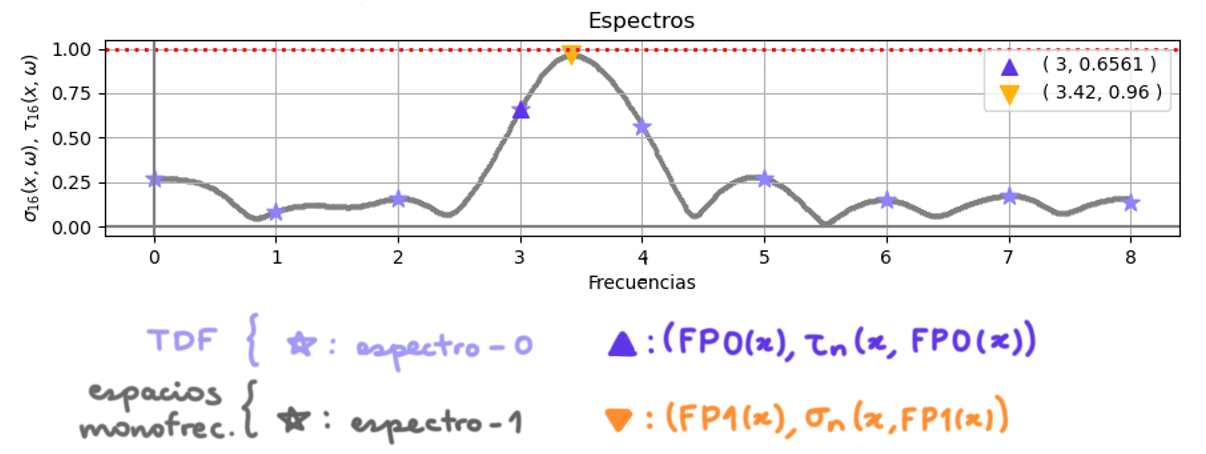
\includegraphics[scale = 1]{./estudios_espectrales/ejemplo_comparacion_1}
\end{figure}


Observe cómo el espectro-$1$ parece completar la información
dada por el espectro-$0$, pues, a diferencia del primero,
el espectro-$0$
da coeficientes de frecuencia $\tau_{n}(x, \omega)$ sólo
para algunas frecuencias enteras $\omega$, mientras que en el espectro-$1$
es posible considerar cualesquiera frecuencias $\omega \geq 0$; como puede observar
en la gráfica, 
\[
FP0 (x) = 3 \hspace{0.2cm} \textit{y} \hspace{0.2cm}
FP1 (x) = 3.42;
\]
esta segunda frecuencia es mucho más cercana a
la frecuencia $\omega =3.4$ del sinusoide del que
fue obtenida la señal $x$; como agregamos ruido
aleatorio en las mediciones, no 
es de extrañarse que no se haya
obtenido exactamente $FP1(x) = 3.4$.

A pesar de que el espectro-$0$, el obtenido a partir de la
transformada discreta de Fourier, no dio una mala estimación (del rango
de frecuencias $Dom_{TDF,n}$ considerado por esta herramienta,
$\omega =3$ es el valor más cercano al valor real $\omega = 3.4$), vemos en este
ejemplo que usando el espectro-$1$ es posible obtener mejores
estimaciones de frecuencias que modelen a la señal original. \\

Mostramos ahora la gráfica de $x$ junto con
\begin{itemize}
	\item la parte de la síntesis de $x$ respecto a la $TDF$
	que corresponde a la frecuencia principal
	$FP0(x)$ (c.f.
	nota \ref{nota: ya?}), que de hecho,
	según la nota \ref{nota: proyeciones monof TDF}, es
	$\Pi_{P_{36,3}}(x)$
	\begin{figure}[H]
			\sidecaption{
			Puesto que $\{ c_{36, 3}, s_{36, \omega} \}$
			es una BON de $P_{36, 3}$, claro que la señal 
			que resulta de discretizar el sinusoide morado en la malla
			$I_{36}$ es, de hecho, la proyección de $x$ 
			al espacio monofrecuencial $P_{36, 3}$.
 			\label{fig: comparacion 2}
			}
			\centering
			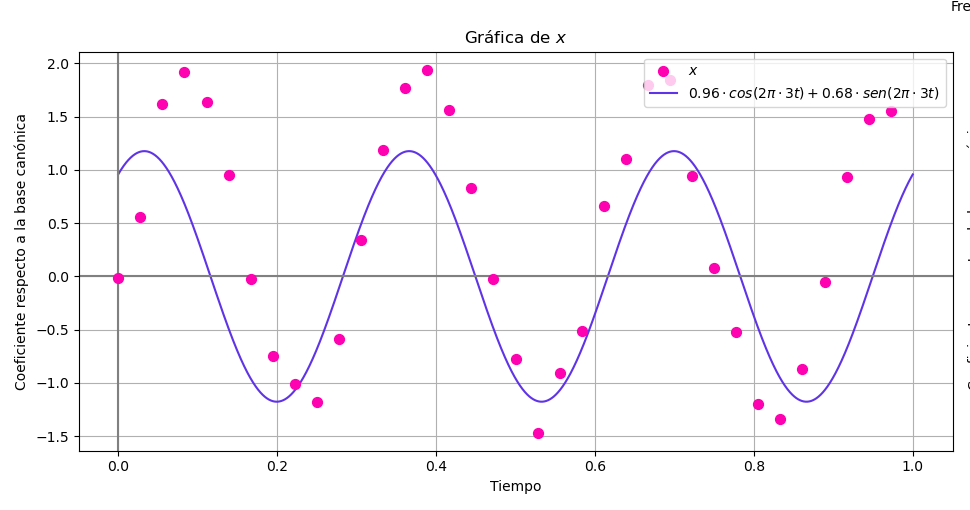
\includegraphics[scale = 0.5]{./estudios_espectrales/ejemplo_comparacion_2} 
		\end{figure}		
	
	y
	\item la señal $\Pi_{P_{16, 3.42}}(x)$, o sea, la señal de
	dimensión $16$ y frecuencia $FP1(x)=3.42$ más cercana a $x$, junto con
	el sinusoide continuo del que fue muestreado.
	\begin{figure}[H]
			\sidecaption{
			Para obtener la versión continua del sinusoide 
			discreto $\Pi_{P_{36, 3.42}}(x)$ (i.e. la gráfica naranja),
			usamos las fórmulas establecidas en los teoremas
			\ref{teo: amelie1} y \ref{teo: amelie2}.
			\label{fig: comparacion 3}
			}
			\centering
			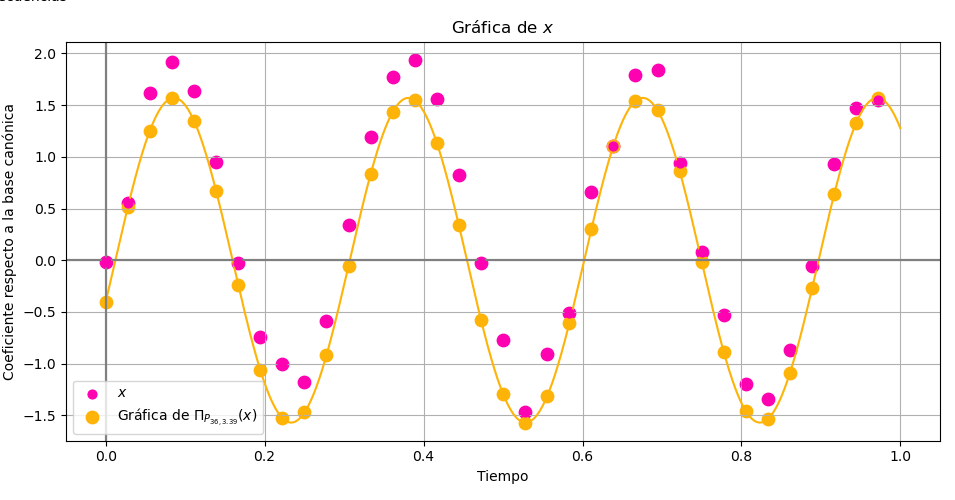
\includegraphics[scale = 0.5]{./estudios_espectrales/ejemplo_comparacion_3} 
		\end{figure}		
\end{itemize}


Los sinusoides de las figuras \ref{fig: comparacion 2} y
\ref{fig: comparacion 3}
son las señales de frecuencia pura
$3$ y $3.42$, respectivamente, cuya distancia euclidea
a la señal original $x$ es mínima. Observe que la segunda
señal, aquella cuya frecuencia
fue determinada
a partir del estudio espectral basado en espacios
monofrecuenciales,
parece ajustarse un poco mejor a la gráfica de $x$. \\

\begin{figure}[H]
			\sidecaption{
			Mostramos ahora los espectros de la señal $x$ que se obtiene
			tomando $36$ muestras uniformemente espaciadas del mismo sinusoide
			$f_{3.4}(t)$, 	
			esta vez sin agregar ruido aleatorio a las mediciones.
			Observe que el espectro-1 detectó a la frecuencia $\omega = 3.4$
			como la mejor, y que el sinusoide naranja ajusta perfectamente la gráfica
			de $x$. Como la frecuencia real no es entera, usar la frecuencia principal
			dada por la TDF sigue sin dar resultados perfectos, aunque no malos.
			\label{fig: sinusoide sin ruido}
			}
			\centering
			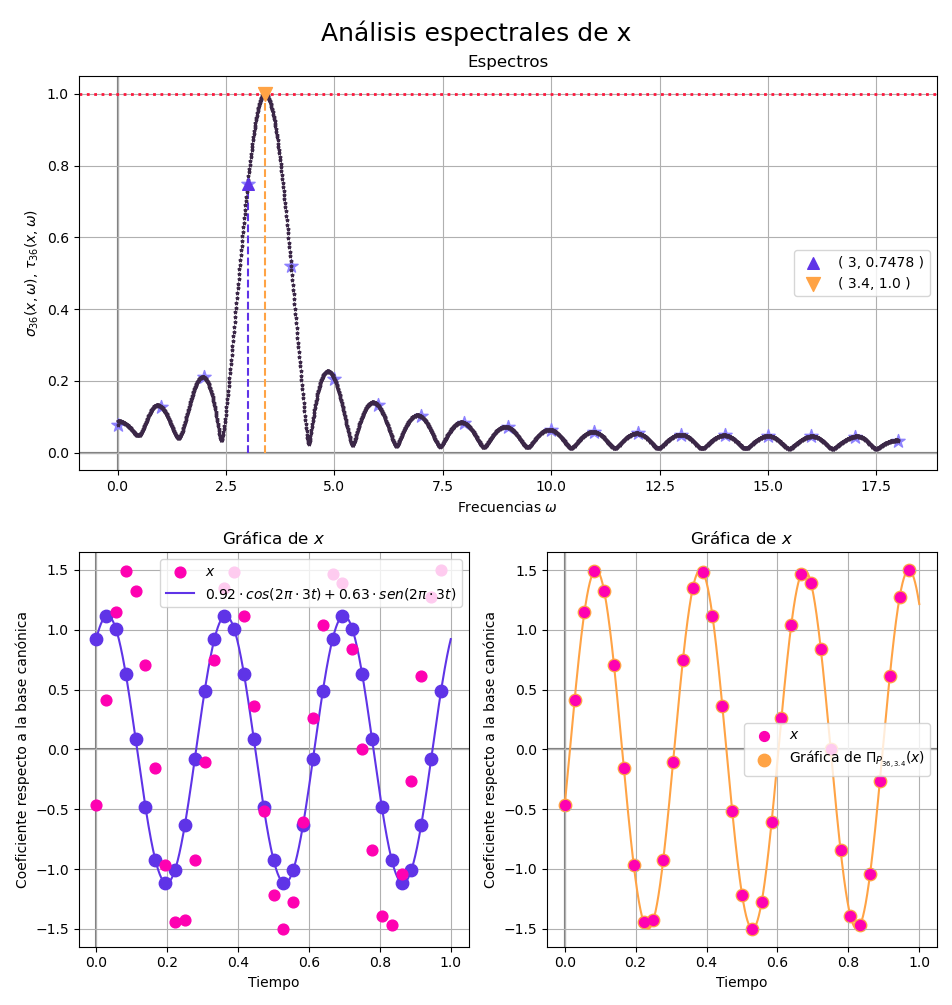
\includegraphics[scale = 0.4]{./estudios_espectrales/sinusoide_sin_ruido} 
		\end{figure}		



	\begin{figure}[H]
			\sidecaption{
			Si ahora muestreamos sin ruido
			del sinusoide $f_{5}$,
			como 
			era de esperarse, la frecuencia principal de ambos
			espectros es $5$
			(y el valor de los 
			espectros en tal frecuencia
			es igual a $1$, la cota
			superior). Además, 
			las gráficas de frecuencia $5$ que resultan
			ajustan a la perfección a la señal original $x$.
			\label{fig: comparacion 4}
			}
			\centering
			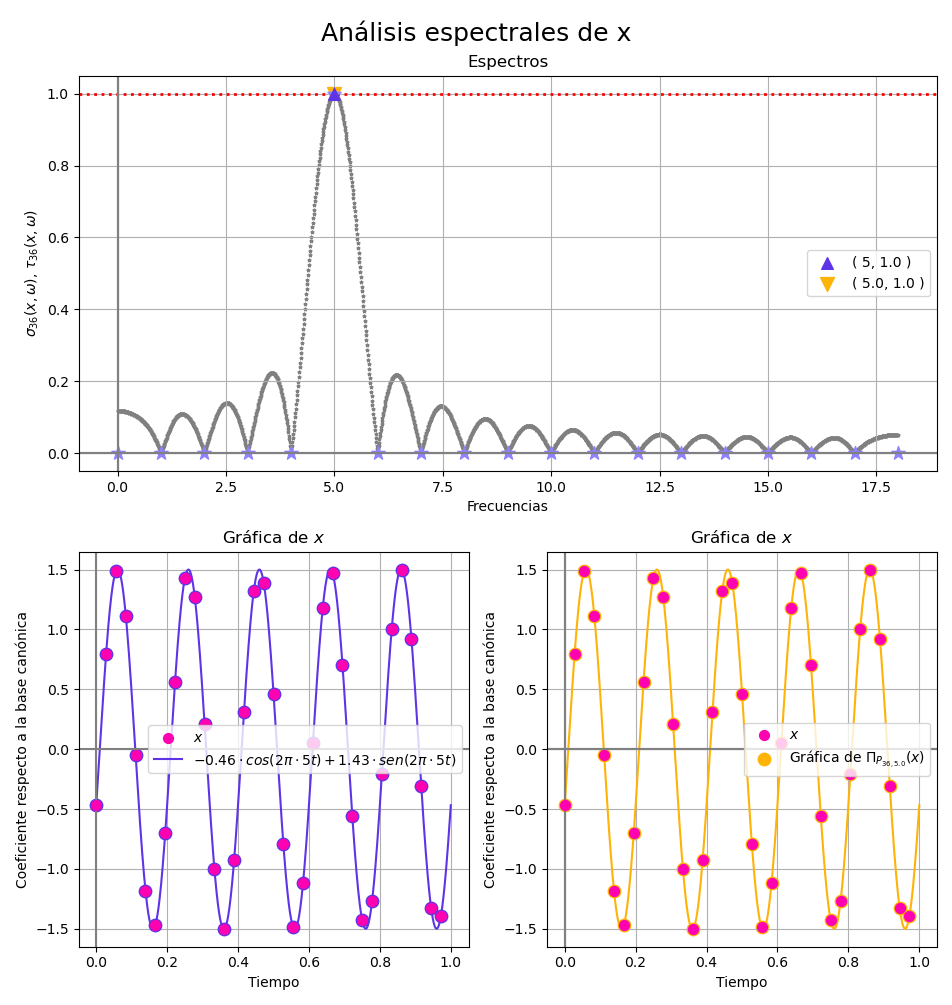
\includegraphics[scale = 0.4]{./estudios_espectrales/ejemplo_comparacion_4} 
		\end{figure}	


Para terminar este ejemplo, tomemos una suma de sinusoides
de varias frecuencias, digamos, de frecuencias
$1$, $4$ y $7$; sea
\[
g(t) = 3 sen(2 \pi t) + sen(2 \pi \cdot 4t) + 0.5 cos(2 \pi \cdot 7t).
\]
Sea $x$ la señal que resulta de muestrar, sin ruido, este sinusoide
$g$, siendo $25$ el tamaño de la muestra.
\begin{figure}[H]
	\sidecaption{
	En la imagen se muestran los espectros de tal $x$. Observe que los
	espectros parecen concentrarse alrededor de las 
	frecuencias $1$, $4$ y $7$.
	\label{fig: sin varias frec}
	}
	\centering
	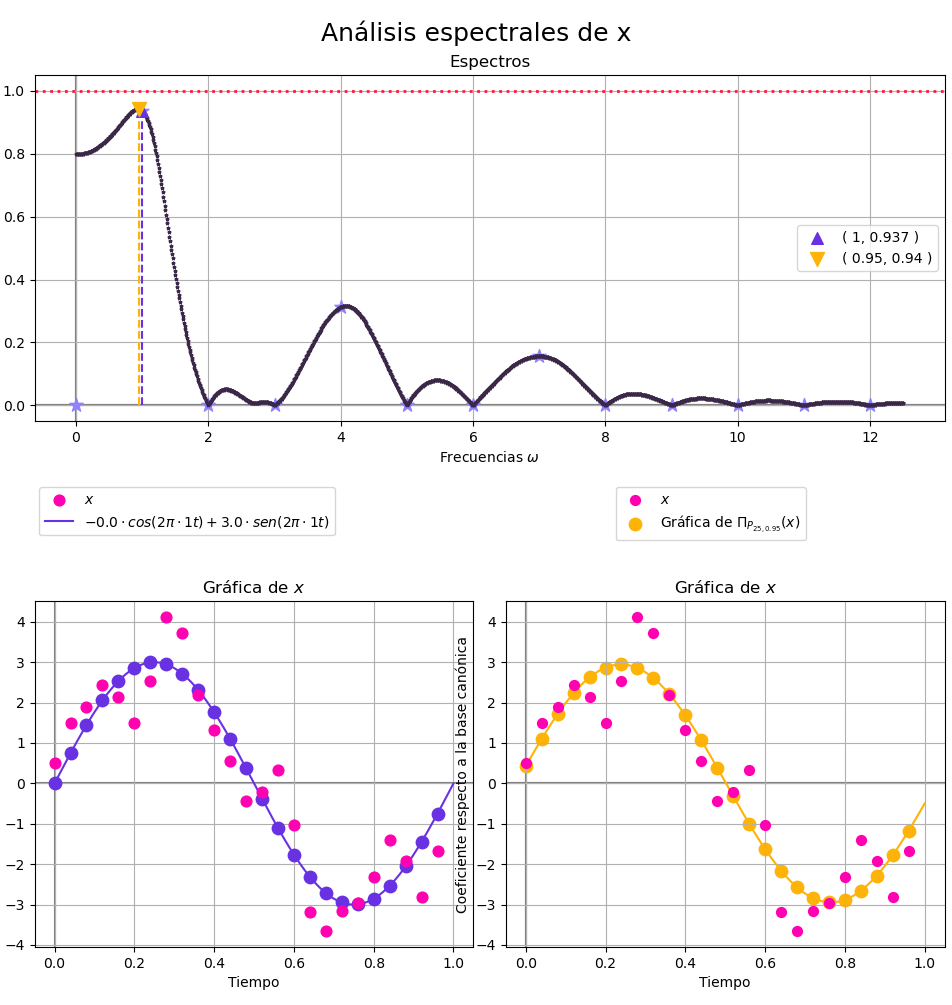
\includegraphics[scale = 0.4]{./estudios_espectrales/sinusoide_varias_frecuencias} 
\end{figure}	

\final
\end{ejemplo}

\subsection{Adaptación del análisis espectral a señales reales con una frecuencia de muestreo dada}

Para hacer nuestros análisis espectrales, hemos
usado la dimensión $n$ del PDL $\cali{L}^{n, k} \in \IR^{n}$
en cuestión
para buscar, en base a máximos globales
del espectro 
$\Sigma_{x}: [0, \frac{n}{2}] \longrightarrow [0,1]$, la
mejor frecuencia $\omega$ para aproximar la gráfica
de $\cali{L}^{n,k}$ en base a un sinusoide discreto
de dimensión $n$. \\


Note que en esa discusión nunca hablamos de 
parámetros importantes para, de forma canónica, hacer
un análisis espectral, como lo son la
duración en tiempo de la señal o la frecuencia
de muestreo.

\begin{defi}
\label{def: tiempo y frec de muestreo}
La cantidad de muestras tomadas (de forma uniforme)
de una señal por unidad de tiempo 
será denotada por $F_{s}$ y llamada \textbf{frecuencia
de muestreo} de la señal. A la cantidad de unidades de
tiempo que dura la medición se le denotará por $T$. \\

A la cantidad total de muestras tomadas se le denotará
por $L$.
\end{defi}
Observe que, para poder dividir una unidad
de tiempo en $F_{s}$ subintervalos de igual longitud,
se deben divider al eje del tiempo con los puntos
\begin{equation}
t_{k} := t_{0} + h k, \hspace{0.2cm}
\textit{con } h := \frac{1}{F_{s}}.
\end{equation}
A tal constante $h$, definida como el recíproco de la frecuencia
de muestreo, se le llama el \textbf{paso temporal} de la señal. \\

De las definiciones se sigue de inmediato que
\begin{equation}
\label{eq: relacion L, T Fs}
L = T F_{s}.
\end{equation}
\begin{figure}[H]
	\sidecaption{
	Adoptamos la convención de empezar a medir 
	un bloque de $F_{s}$ mediciones desde que inicia la
	unidad de tiempo (que, en el caso de la figura, se ha
	fijado como segundos).
	\label{fig: Fs 1}
	}
	\centering
	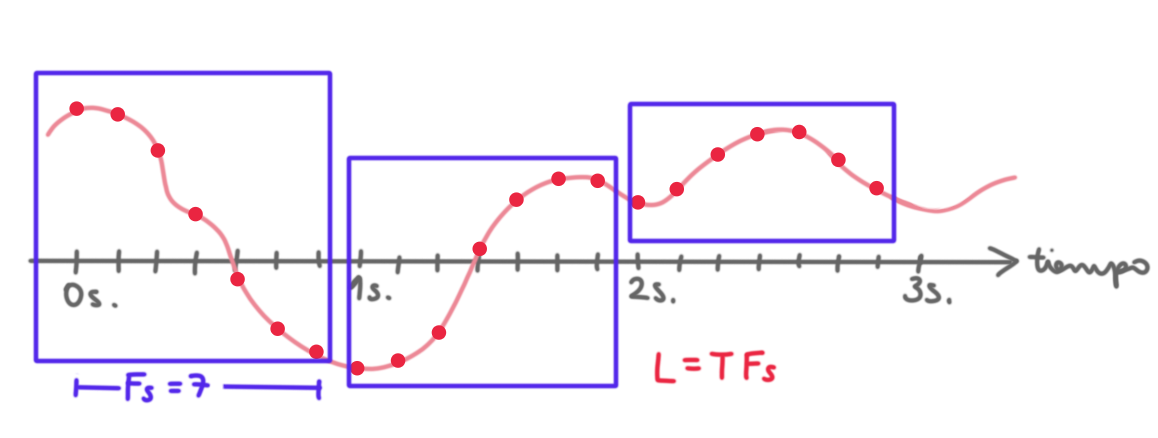
\includegraphics[scale = 1]{Fs_1} 
\end{figure}	

Nosotros, por el momento, sólo nos
hemos enfocado en buscar
una frecuencia $\omega \in [0, \frac{n}{2}]$ que de lugar
a un sinusoide que aproxime bien la gráfica
de $\cali{L}^{n,k}$;
observe que, al hacer esto, hemos supuesto de forma
implícita que estamos estudiando una señal
de duración una unidad de tiempo
($T = 1$) de longitud $n$
(o sea, $L = F_{s} = n$). \\
Supongamos ahora que
tenemos una señal $x$ que consta de $L$ mediciones, siendo
$F_{s}$ la frecuencia de muestreo.
\begin{figure}[H]
	\sidecaption{
	Para la imagen, hemos fijado $F_{s}= 10$
	y $L = 40$.
	\label{fig: frecuencia 1}
	}
	\centering
	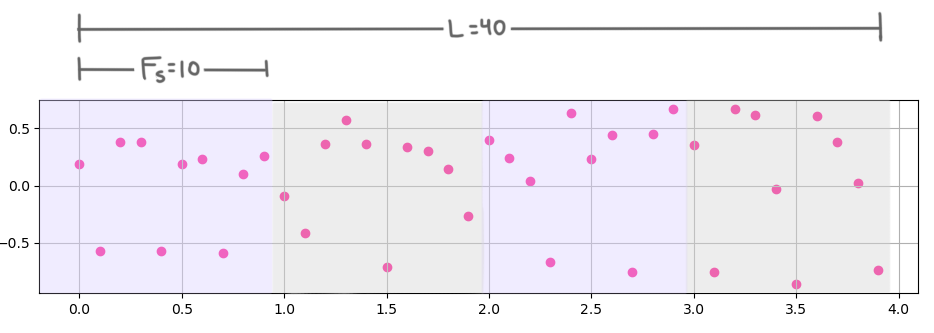
\includegraphics[scale = 0.45]{frecuencia_1} 
\end{figure}	

Sea ahora $2 \leq n \leq L$ y
supogamos que
se hizo el análisis
espectral 
de una sección $x_{|n}$ de tal señal
que conste de $n$ puntos
(usando el espectro
$\Sigma_{x}: [0, \frac{n}{2}]
\longrightarrow [0,1]$).
Digamos que, como conclusión de ese análisis, se
obtuvo que un sinusoide de frecuencia $\omega \in [0, \frac{n}{2}]$
ajusta bien \textit{esa sección particular 
$x_{|n}$
de la señal $x$}.
\begin{figure}[H]
	\sidecaption{
	Para la imagen, hemos fijado $n= 6$;
	se calculó que la mejor frecuencia para ajustar 
	los primeros $6$ puntos que componen la señal
	original $x$ es $w = 2$.
	\label{fig: frecuencia 2}
	}
	\centering
	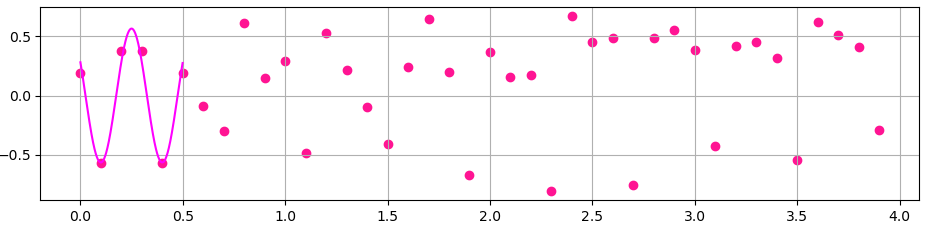
\includegraphics[scale = 0.45]{frecuencia_2} 
\end{figure}	

Observe que, en general, si se quisiera usar
directamente una frecuencia de $w$ para ajustar
a la señal $x$, la aproximación lograda en los
$n$ puntos escogidos previamente puede no ser válida.
\begin{figure}[H]
	\sidecaption{
	Usando los datos de la figura \ref{fig: frecuencia 2}, podriamos
	intentar en un principio usar a un sinusoide de frecuencia $2$
	para intentar modelar a la señal, pero un sinusoide de tal frecuencia,
	como es el caso de esta figura, puede que ni siquiera sea adecuado
	para modelar el pedazo $x_{|n}$ original a partir del cual se obtuvo
	la frecuencia $\omega$.
	\label{fig: frecuencia 2}
	}
	\centering
	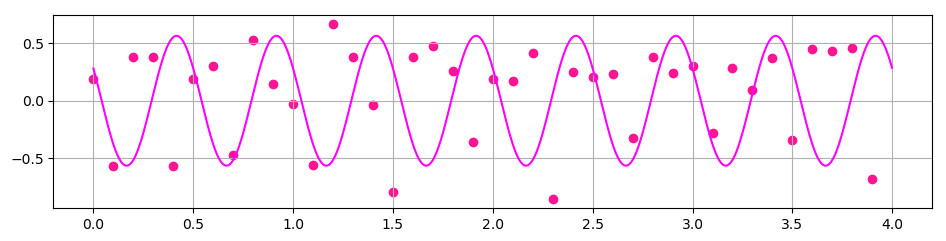
\includegraphics[scale = 0.45]{frecuencia_3} 
\end{figure}
Esto se debe a que	
tal frecuencia $\omega$ es buena para aproximar
a dichos $n$ puntos cuando se ha tomado como
unidad de tiempo a $n$, pero, 
por la forma en que fue muestreada la señal original $x$,
son $F_{s}$ (y no necesariamente $n$) la cantidad de puntos
que conforman una unidad. Así, puesto que con $\omega$
ciclos de un sinusoide se aproximaron $n$ puntos, 
la frecuencia que debe escogerse para aproximar a todos los $L$
puntos es
\begin{equation}
\label{eq: rel frecuencia real y ficticia}
\tilde{w} := \frac{F_{s}}{n} \omega.
\end{equation}

\begin{figure}[H]
	\sidecaption{
	Es con una simple regla de tres que se deduce
	la relación \eqref{eq: rel frecuencia real y ficticia}.
	\label{fig: frecuencia real}
	}
	\centering
	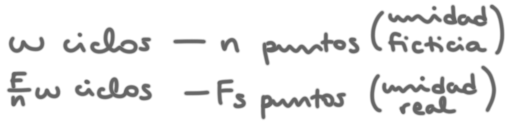
\includegraphics[scale = 1.4]{frecuencia_real} 
\end{figure}	
\begin{figure}[H]
	\sidecaption{
	Según los datos de las figuras
	\ref{fig: frecuencia 1}
	y \ref{fig: frecuencia 2}, con un sinusoide de frecuencia
	$\tilde{\omega} = 10/3$ se aproximan bien a los seis
	puntos en base a los cuales se encontró a la primera
	frecuencia $\omega$.
	\label{fig: frecuencia 4}
	}
	\centering
	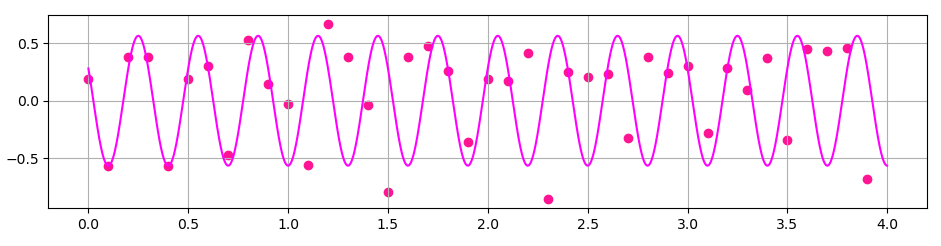
\includegraphics[scale = 0.45]{frecuencia_4} 
\end{figure}
\section{PROVISIONAL; límites}

En \TODO{rojo} se resaltan las fórmulas que YA se han
verificado calculándolas dos veces. En 
\textcolor{blue}{azul} cuando la aproximación ha sido
simulada exitosamente.


\TODO{
\[
\frac{sen(2 \pi \omega) cos(2 \pi \omega \frac{n-1}{n})}{sen
(2 \pi \frac{\omega}{n})}
\sim
\frac{
2 \pi \omega - \frac{4 \pi^{3}}{3n^{2}}
(4n^2-6n+3) \omega^{3} + o(\omega^{5})
}{
\frac{2\pi}{n} \omega -
\frac{4 \pi^{3}}{3 n^{3}} \omega^{3} + o(\omega^{5})
},
\]
}
por lo que

\textcolor{blue}{
\begin{align*}
\xi_{n, \omega} \sim &
\sqrt{2} 
\left(
4 \pi
\frac{                                                                                                                                          
\omega - \frac{2\pi^{2}}{3n^{2}}(2n^2-3n+2)\omega^{3} + o(\omega^{5})
}{
\frac{2\pi}{n} \omega -
\frac{4 \pi^{3}}{3 n^{3}} \omega^{3} + o(\omega^{5})
}
\right)^{-1/2} \\
\sim &
\sqrt{2} 
\left(
2n
\frac{                                                                                                                                          
\omega - \frac{2\pi^{2}}{3n^{2}}(2n^2-3n+2)\omega^{3} + o(\omega^{5})
}{
\omega -
\frac{2 \pi^{2}}{3 n^{2}} \omega^{3} + o(\omega^{5})
}
\right)^{-1/2} 
\rightarrow \frac{1}{\sqrt{n}},
\end{align*}
}

\textcolor{blue}{
\begin{align*}
\eta_{n, \omega} \sim &
\sqrt{2} 
\left(
\frac{
8 \pi^{3} (2n-1)(n-1)\omega^{3} + o(\omega^{5})
}{
6 \pi n \omega -
\frac{4 \pi^{3}}{n} \omega^{3} + o(\omega^{5})
}
\right)^{-1/2} \\
\sim & 
\sqrt{2} 
\left(
4\pi^{2}
\frac{
(2n-1)(n-1)\omega^{3} + o(\omega^{5})
}{
3 n \omega -
\frac{2 \pi^{2}}{n} \omega^{3} + o(\omega^{5})
}
\right)^{-1/2} 
 \rightarrow \infty.
\end{align*}
}

\textcolor{blue}{
\begin{align*}
\langle
c_{n, \omega}, s_{n, \omega}
\rangle \sim &
\frac{2\pi}{n}
\xi_{n, \omega} \eta_{n, \omega}
(n-1)  
\left(
\frac{n}{2} \omega - \frac{2\pi^{2}}{3} (n-1) \omega^{3} + o(\omega^{5})
\right) \\
= & 
\frac{2 \sqrt{2}}{n \sqrt{n}} \pi (n-1)
\left(
\frac{
\frac{3}{2} \pi n^{3}\omega^{3} + o(\omega^{5})
}{
8 \pi^{3}(2n-1)(n-1)\omega^{3} + o(\omega^{5})
}
\right)^{1/2}
\rightarrow \frac{
\sqrt{6(n-1)}
}{2 \sqrt{2n-1}}.
\end{align*} 
}
Tuve que usar la expresión asintótica
de $\eta_{n, \omega}$ para poder determinar este
último límite, pues con la expresión de la
primera linea tenía una indeterminación
de tipo $\infty \cdot 0$.

\textcolor{blue}{
\[
\langle x,
c_{n, \omega}
\rangle = 
\xi_{n, \omega} 
\left(
X_{0} - \frac{2 \pi^{2}}{n^{2}}X_{2} \omega^{2} 
+ \frac{2 \pi^{4}}{3n^{4}} X_{4} \omega^{4} + o(\omega^{5})
\right) \rightarrow \frac{X_{0}}{\sqrt{n}} ,
\]
}

\textcolor{blue}{
\begin{align*}
\langle x,
s_{n, \omega}
\rangle = &
\eta_{n, \omega} 
\left(
\frac{2 \pi}{n} X_{1} \omega - \frac{4 \pi^{3}}{3n^{3}}X_{3} \omega^{3} 
 + o(\omega^{5})
\right)\\
= &
\begin{cases}
\sqrt{2} \left(
\frac{
\frac{24 \pi^{3}}{n}X_{1}^{2}\omega^{3} + o(\omega^{5}) }{
8 \pi^{3} (2n-1)(n-1)\omega^{3} + o(\omega^{5})
}
\right)^{1/2}
\rightarrow \left(
\frac{6 X_{1}^{2}}{(2n-1)(n-1)n}
\right)^{1/2} & \textit{si } \alpha_{n, \omega}(x) \geq 0 \\
-\sqrt{2} \left(
\frac{
\frac{24 \pi^{3}}{n}X_{1}^{2}\omega^{3} + o(\omega^{5}) }{
8 \pi^{3} (2n-1)(n-1)\omega^{3} + o(\omega^{5})
}
\right)^{1/2}
\rightarrow -\left(
\frac{6 X_{1}^{2}}{(2n-1)(n-1)n}
\right)^{1/2} & \textit{si } \alpha_{n, \omega}(x) < 0,\\
\end{cases}
\end{align*}
}
donde
\[
\alpha_{n, \omega}(x) := 
\frac{2 \pi}{n} X_{1} \omega - \frac{4 \pi^{3}}{3n^{3}}X_{3} \omega^{3}.
\] 

\TODO{Ya lo tengo. Lo único no tan lindo de la fórmula
es que se requiere calcular el signo del coeficiente alpha. No sé si 
sea siempre fácil de determinar-o si quiera
si sea constante cerca de cero. Lo que yo hice en el programa es determiar
el signo para cuando $\omega = 0.001$}





\begin{equation}
\label{ec: limite x, cnw}
\limite{\omega \rightarrow 0^{+}}{\langle
x, c_{n, \omega}
\rangle }
= \frac{X_{0}}{\sqrt{n}}
\end{equation}

\begin{equation}
\label{ec: limite x, snw}
\limite{\omega \rightarrow 0^{+}}{\langle
x, s_{n, \omega}
\rangle }
\begin{cases}
\left(
\frac{6 X_{1}^{2}}{(2n-1)(n-1)n}
\right)^{1/2} & \textit{si } \alpha_{n, \omega}(x) \geq 0 \\
-\left(
\frac{6 X_{1}^{2}}{(2n-1)(n-1)n}
\right)^{1/2} & \textit{si } \alpha_{n, \omega}(x) < 0,\\
\end{cases}
\end{equation}

\begin{equation}
\label{ec: limite -2abc}
\limite{\omega \rightarrow 0^{+}}{
-2 \langle x, c_{n, \omega} \rangle
\langle x, s_{n, \omega} \rangle
\langle c_{n, \omega}, s_{n, \omega} \rangle
= 
}
\end{equation}

Así, los elementos que parecen en la fórmula
para $\sigma_{n}(x, \omega)$ cuando $\omega \not\in \frac{n}{2} \IZ$ son
\begin{itemize}
\item 
\TODO{
\[
\langle
c_{n, \omega}, s_{n, \omega}
\rangle^{2} \sim
\frac{4\pi^{2}}{n^{2}}(n-1)^{2} \xi_{n, \omega}^{2} \eta_{n, \omega}^{2}
\left(
\frac{n^{2}}{4} \omega^{2} - \frac{2n}{3} \pi^{2} (n-1) \omega^{4} + o(\omega^{5})
\right)
\]
}
sigue desarrollando el eta  !!!
\item
\TODO{
\[
\langle x,
c_{n, \omega}
\rangle^{2} = 
\xi_{n, \omega}^{2}
\left(
X_{0}^{2} - \frac{4 \pi^{2}}{n^{2}}X_{0}X_{2} \omega^{2} 
+ 
\frac{4 \pi^{4}}{n^{4}}
\left(
\frac{1}{3} X_{0}X_{4} + X_{2}^{2}
\right) \omega^{4} 
+ o(\omega^{5})
\right)
\]
}

\item
\TODO{
\[
\langle x,
s_{n, \omega}
\rangle^{2} = 
\frac{4 \pi^{2}}{n^{2}}
\eta_{n, \omega}^{2}
\left(
X_{1}^{2}\omega^{2} - \frac{4 \pi^{2}}{3n^{2}}X_{1}X_{3} \omega^{4} 
+  o(\omega^{5})
\right)
\]
}

\item
\[
\langle
x, c_{n, \omega}
\rangle
\langle
x, s_{n, \omega}
\rangle
\langle
c_{n, \omega}, s_{n, \omega}
\rangle \sim
\frac{2 \pi^{2}}{n}
\xi_{n, \omega}^{2} \eta_{n, \omega}^{2}(n-1)
\left(
X_{0}X_{1}\omega^{2} 
- \frac{2 \pi^{2}}{n}
\left(
\frac{1}{3n} X_{0}X_{3} + \frac{1}{n} X_{2}X_{1}
+ \frac{2}{3}(n-1)X_{0}X_{1}
\right) \omega^{4}
\right).
\]
\end{itemize}

\TODO{Cambia los iguales por $\sim$.}
Según estos cálculos, si
$a_{n, \omega} = \langle x, c_{n, \omega} \rangle$, 
$b_{n, \omega} = \langle x, s_{n, \omega} \rangle$, 
$c_{n, \omega} = \langle c_{n, \omega}, s_{n, \omega} \rangle$, 
entonces

\[
a_{n, \omega}^{2} + b_{n, \omega}^{2} - 
2a_{n, \omega}b_{n, \omega}c_{n, \omega}
= N_{1} + N_{2} +N_{3},
\]
donde

\[
N_{1} =
\xi_{n, \omega}^{2} \left(
X_{0}^{2} - \frac{4\pi^{2}}{n^{2}} X_{0}X_{2}
\omega^{2} + \frac{4 \pi^{4}}{n^{4}}
\left(
\frac{1}{3} X_{0}X_{4} + X_{2}^{2}
\right) \omega^{4}
\right)
\rightarrow 
\frac{X_{0}}{n}
\left(
X_{0}  - \frac{4 \pi^{2}}{n^{2}}X_{2}
\right),
\]

\[
N_{2} = \frac{4 \pi^{2}}{n^{2}} \eta_{n, \omega}^{2}
\left(
X_{1}^{2} \omega^{2} - \frac{4 \pi^{2}}{3n^{2}}X_{1}X_{3} \omega^{4}
+ o(\omega^{5})
\right)
=
\frac{16 \pi^{3}}{n^{2}}
\frac{3n \omega - \frac{2 \pi^{2}}{n} \omega^{3} + o(\omega^{5})}{
8 \pi^{3}(2n-1)(n-1) \omega^{3} + o(\omega^{5})
}
\rightarrow \infty,
\]

\[
N_{3} =
\frac{-4 \pi^{2}}{n}
\xi_{n, \omega}^{2} \eta_{n, \omega}^{2}(n-1)
\left(
X_{0}X_{1}\omega^{2} 
- \frac{2 \pi^{2}}{n}
\left(
\frac{1}{3n} X_{0}X_{3} + \frac{1}{n} X_{2}X_{1}
+ \frac{2}{3}(n-1)X_{0}X_{1}
\right) \omega^{4}
\right)
\rightarrow ?,
\]
luego, no puedo determinar este último límite, por lo tanto,
tampoco hablar solbre el límite de
de $a_{n, \omega}^{2} + b_{n, \omega}^{2} - 
2a_{n, \omega}b_{n, \omega}c_{n, \omega}$, pues
tengo una indeterminación del tipo 
$0 \cdot \infty$. \\

El denominador es
\[
1-c^{2} \sim
1 - \frac{4\pi^{2}}{n^{2}}(n-1)^{2} \xi_{n, \omega}^{2} \eta_{n, \omega}^{2}
\left(
\frac{n^{2}}{4} \omega^{2} - \frac{2n}{3} \pi^{2} (n-1) \omega^{4} + o(\omega^{5})
\right) \rightarrow ?,
\]
aquí también tengo una indeterminación de tipo
$0 \cdot \infty$.

